\documentclass[border=10pt]{standalone}
\usepackage{pgfplots}
\pgfplotsset{compat=1.18}

\begin{document}
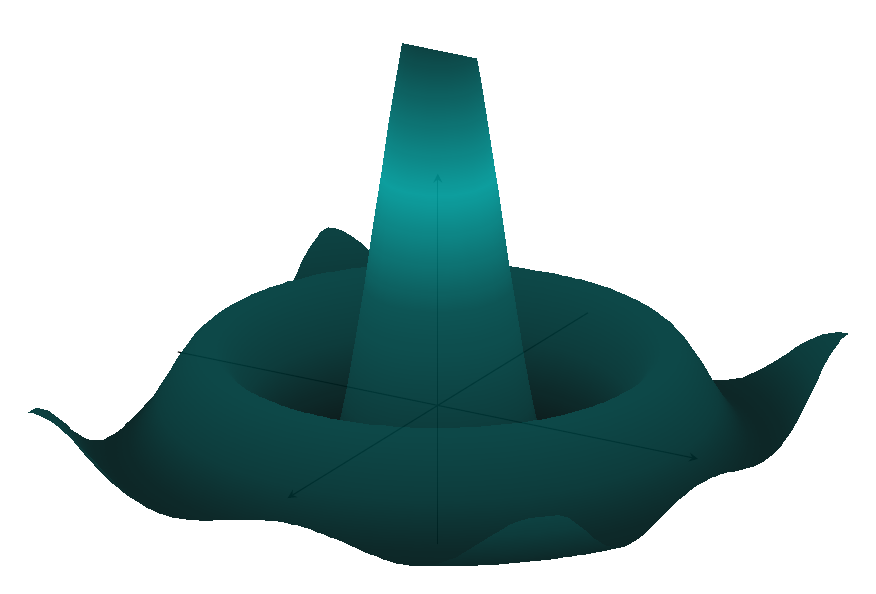
\begin{tikzpicture}
\begin{axis}[
    view={120}{30},
    width=12cm,
    height=10cm,
    grid=major,
    xlabel={},
    ylabel={},
    zlabel={},
    xmin=-5, xmax=5,
    ymin=-5, ymax=5,
    zmin=-0.3, zmax=0.5,
    xtick={-4,-2,0,2,4},
    ytick={-4,-2,0,2,4},
    ztick={-0.2,0,0.2,0.4},
    colormap={tealwave}{
        color=(black) 
        color=(teal!40!black) 
        color=(teal!60!black) 
        color=(teal!80!cyan) 
        color=(teal!60!black)
        color=(black)
    },
    shader=interp,
    samples=80,
    domain=-5:5,
    y domain=-5:5,
    axis lines=middle,
    axis on top=false,
    tick style={draw=none},
    xticklabels={},
    yticklabels={},
    zticklabels={},
]

\addplot3[
    surf,
    opacity=0.95,
    faceted color=none,
    point meta=z,
] 
{(x^2 + y^2 < 0.01) ? 0.4 : (sin(deg(sqrt(x^2+y^2)*2))/sqrt(x^2+y^2)/2)};

\end{axis}
\end{tikzpicture}
\end{document}